%%%% Implementation/Eval section

\section{Monitor Implementation}
\subsection{Evaluation}
\label{sec:eval:embedded}
To evaluate the embedded monitor we need to check an actual CAN bus.  
Since we did not have current access to a real system with CAN and a data dictionary to monitor, we instead performed real-time replay of timestamped CAN logs captured during testing of a real system onto a bench CAN bus which the monitor was connected to, as shown in Figure \ref{fig:eval:replaySchem}. 

\begin{figure}
\centering
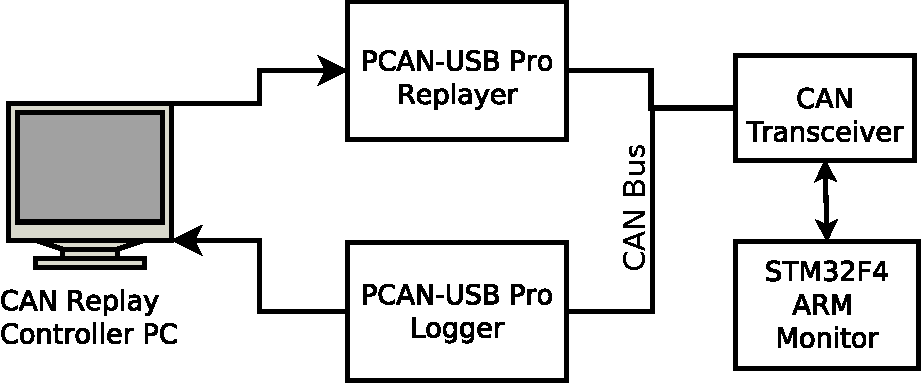
\includegraphics[width=4.5in]{img/replay_arch}
\caption{CAN replay setup \label{fig:eval:replaySchem}}
\end{figure}
%%% about SUT
The system under test that provided the logs is an autonomous heavy truck which is being designed for use in vehicle platoons. % cite/discuss AMAS/ASTAA?
The system has multiple internal buses, some CAN and some Ethernet, connecting different system components. We utilize logs from the CAN bus connecting the primary vehicle controller and the user interface controller because it provides a reasonable amount of observable state which maps to actual system requirements which we can monitor.
%
%The logs we monitor are from robustness testing of the interface controller, so we focus on its CAN bus which contains communication between the interface controller and the primary vehicle controller.
The logs contain both normal operation as well as some operation under network-based robustness testing. During robustness testing, the testing framework can hijack targeted network messages on the bus to inject testing values. % could cite astaa here

A PC was connected to a PCAN-USB Pro \cite{PCAN-USBPro} device which provides a USB interface to two CAN connections. One CAN channel was used as the log replayer, while the other was used as a bus logger for analysis purposes.
%%%@RV cutting for space, RV people probably don't care about these specifics too much
%%% replay
%We performed log replay with a PC-based script which would take a test log and replay it on the CAN bus based on the log's timestamps. A separate script used the second CAN connection to log the CAN network traffic.
%The replay timing is based on a busy-wait using the log timestamps. 
%We compared the replayed log timings to the original test logs to ensure this replay was accurate. 
%The percent error in message timestamps relative to the start of the message in our longest logs had an average of less than 0.01\% error. The absolute error was generally sub-millisecond, which is accurate enough for our 25ms monitor with its greater than 50ms minimum time step resolution.

%Figure \ref{fig:eval:replay_timing} compares the replayed log timings to the actual test logs.
%D%\begin{table}
%D%\centering
%D%\begin{tabular}{|l|l|l|}
%D%\hline Log \# & Average delta error & average message error \\
%D%\hline 1 & -0.0005\% & \\
%D%\hline 2 & -0.00499\% & \\
%D%\hline
%D%\end{tabular}
%D%\caption{CAN Log Replay Timing Error}
%D%\label{tab:eval:replay_timing}
%D%\end{table}


%%%%%%%%%
%% rule elicitation
\subsection{Monitor Specification}
\label{sec:monspec}
Requirements documentation for this system was available, so we were able to build a monitoring specification based on actual system requirements.
%For this system we did have requirements documentation which could more directly lead to a monitoring specification. 
%Due to the test focus for the logs we have, we mainly created specifications checking the user interface feature. 
The specification evaluated in the embedded monitor on the test logs are shown in Table \ref{tab:monspec}. This specification was derived from the system requirements based on the observable system state available in the testing logs.
%Based on the given requirements, the coverage of available test logs, and the observability of the 
%Since we wanted to monitor the interface bus, we identified requirements which we could monitor or partially monitor based on the state available on this bus.
%The specifications we used on the embedded monitor are shown in Table \ref{tab:eval:nrecrules} and the propositions used in these rules are described in Table \ref{tab:eval:nrecprops}.

\begin{table}
%\begin{tabular}{|p{3in}|l|}
\begin{tabular}{|l|p{4.5in}|}
\hline \multirow{2}{*}{Rule \#} & Informal Rule \\ & BMTL \\
%\hline Informal Rule & BMTL \\
%\hline \multirow{2}{*}{0} & A feature heartbeat shall be received every 500ms \\
%& $\lozenge_{[0,100ms]} HeartBeat$ \\
\hline \multirow{2}{*}{0} & A feature heartbeat shall be received every 500ms \\
& $HeartbeatOn \rightarrow \lozenge_{[0,500ms]} HeartBeat$ \\
\hline \multirow{2}{*}{1} & The interface component heartbeat counter is correct \\
& $HeartbeatOn \rightarrow HeartbeatCounterOk$ \\
%% make sure to put both status and command in here (maybe split them)
%\hline \multirow{2}{*}{2} & The vehicle controller shall not command a transition from manual mode to autonomous mode as seen on the interface component \\ 
\hline \multirow{2}{*}{2} & The vehicle shall not transition from manual mode to autonomous mode \\
&  $\neg ((\blacksquare_{[1,1]} IntManualState) \wedge IntAutoStat)$\\
\hline \multirow{2}{*}{3} & The vehicle controller shall not command a transition from manual mode to autonomous mode \\
& $\neg ((\blacksquare_{[1,1]} VehManualModeCmd) \wedge VehAutoModeCmd)$\\
\hline \multirow{2}{*}{4} & The vehicle shall not transition from system off mode to autonomous mode \\ 
&  $\neg ((\blacksquare_{[1,1]} IntSDState) \wedge IntAutoStat)$\\
\hline \multirow{2}{*}{5} & The vehicle controller shall not command a transition from system off mode to autonomous mode \\
& $\neg ((\blacksquare_{[1,1]} VehSDModeCmd) \wedge VehAutoModeCmd)$\\
% warn was at 200ms
\hline
\end{tabular}
\caption{CAN replay monitoring specification \label{tab:monspec}}
\end{table}

The rules were derived from the vehicle safety requirements documentation. 
Limited to the observable state on the interface bus, we used the user interface LEDs as proxies for the actual system state. 
This is an approximation we would feel is reasonable in most systems, and in this case there were also safety requirements which state that the output LEDs should be correct. This provides us more assurance that the approximation is reasonable.

% describe rules
% hb rules
Rule \#0 is a heartbeat detection which ensures that the interface component is still running (essentially a watchdog message). Rule \#1 is a second component of this check. The system's heartbeat message contains a single heartbeat status bit which we checked directly in Rule \#0, but the message also has a rolling counter field. 
We used the semi-formal interface to create a proposition that represents whether the counter is incrementing correctly (i.e., one value at a time). To block false-positive violations during initialization, we blocked these rules from being checked until after the first heartbeat message was received by creating a guard proposition $HeartbeatOn$ with the semi-formal interface. 
%Initialization of the system and monitor's model can be troublesome for monitoring, especially in testing when missing or unfinished components cause the system to take more time to get to a stable, monitorable state.
Initialization issues are discussed in more detail in Section \ref{sec:eval:mon_init}. 

% transition rules
We also watched the system state for illegal state transitions. Although the actual mode decisions and commands are on a different bus, we can still monitor the system state through the user interface LEDs which show the mode state. 
We created rules for two of the illegal transitions, from manual mode to autonomous driving and from system off to autonomous driving. We independently checked both the vehicle controller's LED command messages and the interface's LED status message for these transitions.

% RV prop mappings
The proposition mappings in this system were straightforward. Most of the specification propositions are boolean values taken directly from the network messages. The heartbeat counter is checked with a more complicated mapping that ensures the rolling counter is consistent (i.e., counts up and wraps correctly).

%%@RV cutting for space
%% prop mappings
%The proposition mappings here were straightforward. The LED command and status messages were single bit fields and we checked the heartbeat's single bit status message. We checked the rolling heartbeat counter for  consistency (i.e., that it counted up and wrapped correctly) by comparing it against the previously seen value in the semi-formal interface. We also created the guard $HeartbeatOn$ which is false until the first heartbeat message is seen, and true from then on. 
%% This was necessary to handle initialization issues
%Using a guard proposition is our primary method to implement unbounded since/until type rules within our bounded logic. If we had unbounded operators we could use the formula $(\lozenge_{[0,500]} Heartbeat)\; \mathcal{S}\; (Heartbeat)$ instead of a mode-based guard proposition, but without unbounded operators using guard propositions to enable or disable a formula is a reasonable replacement.
%
%\begin{table}
%\centering
%\caption{CAN replay propositions}
%\label{tab:eval:nrecprops}
%\begin{tabular}{lp{2in}l}
%\textbf{Proposition Name} & \textbf{System Variables} & \textbf{Mapping} \\
%\hline $HeartBeat$ & Feature Status Message Heartbeat field & Fresh direct boolean \\
%$HeartbeatOn$ & Interface HB message & System Mode \\
%$HeartbeatCounterOk$ & Interface HB message & Comparison with Past Value \\
%$VehManualModeCmd$ & Vehicle command message & Direct Boolean \\
%$VehAutoModeCmd$ & Vehicle command message & Direct Boolean \\
%$VehicleSDModeCmd$ & Vehicle command message & Direct Boolean \\
%$IntManualStat$ & Interface status message & Direct Boolean \\
%$IntAutoStat$ & Interface status message & Direct Boolean \\
%$IntSDStat$ & Interface status message & Direct Boolean \\
%\end{tabular}
%\end{table}


%% replay
\subsection{Monitoring results}
We monitored the CAN log replays on our test CAN network with the specification discussed above and found heartbeat violations in the robustness testing logs.
%
% covering all three possible violation types. One was a false positive
Three different types of heartbeat violations were identified after inspecting the monitor results.
% missing hb message
The first is a late heartbeat message. In one of the robustness testing logs the heartbeat message was not sent on time, which is clearly a heartbeat violation. Figure \ref{fig:eval:hb_arrival:vals} shows the heartbeat counter values and the inter-arrival time of the heartbeat messages over time for this violation. We can see here that the heartbeat counter did in fact increment in a valid way, just too slowly. 
%Figure \ref{fig:eval:hb_arrival:time} shows the inter-arrival time of these same messages.

\begin{figure}
	%\begin{subfigure}
		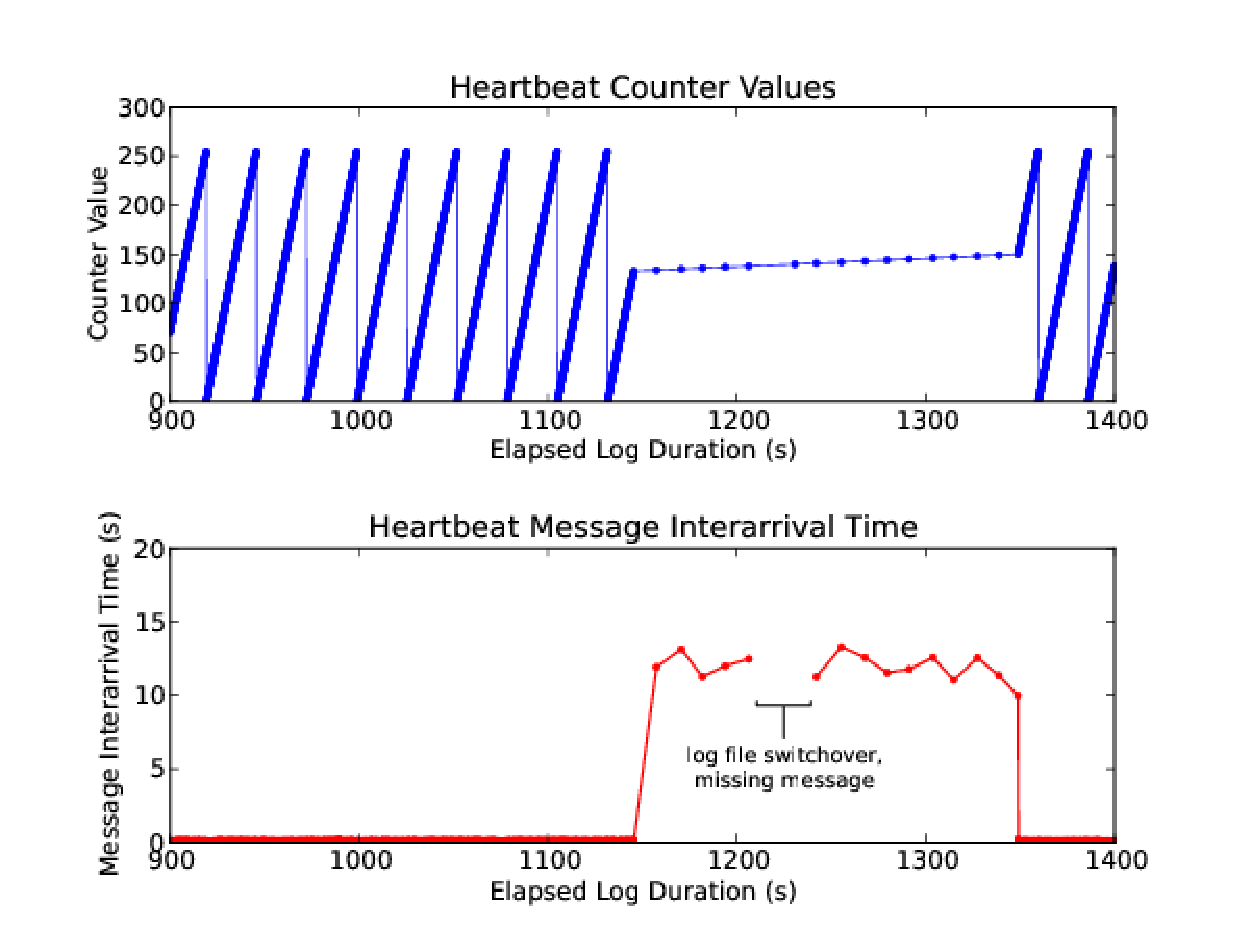
\includegraphics[width=4.5in]{img/hb1}
		%\includegraphics[width=6in]{img/fake_hb1}
		\caption{Heartbeat counter values over time}
		\label{fig:eval:hb_arrival:vals}
	%\end{subfigure}
\end{figure}
%\begin{figure}
%%	\begin{subfigure}
%%		%\includegraphics[width=6in]{img/hb}
%		\caption{Heartbeat counter message inter-arrival time}
%		\label{fig:eval:hb_arrival:time}
%	%\end{subfigure}
%\end{figure}
%%\caption{Bad Heartbeat Log}
%%\end{figure}

% bad status
The second violation is on-time heartbeat status message but the heartbeat status field is 0. 
We do not know from the available documentation whether a bad status in an on-time message with a good counter is valid or not. So without more information we cannot tell whether these violations are false positives or not. This is worthy of further investigation.

% bad counter
The last type of violation is a bad counter. 
We have defined a good counter as one which increments by one every message up to its maximum (255 in this case) before wrapping back to zero.
Every consecutive heartbeat status message must have an incremented heartbeat counter or a violation will be triggered. Figure \ref{fig:eval:hb_badcounter} shows the counter value history for one of the traces with a heartbeat violation caused by a bad counter value.
%
%@EDIT describe robustness testing, define these false positives like the talk?
Further inspection of this violation showed that the bad counter values were sent by the testing framework rather than the actual system. In this case, the network traffic the monitor is seeing is not real system state but actually it is messages being injected by the testing framework. This is not a real violation (since the violating state is not the actual system state), and so we consider this a false positive violation.
% this is a false positive

Different counter restrictions could also be used, such as allowing unchanging as well as incrementing values or requiring an increment to occur within a time threshold rather than every message. Once again, without documentation to point us towards the right restriction, all we can do is try a restriction and after seeing the monitoring results decide whether we believe our restriction is accurate or causes too many false positives. 
\begin{figure}
%includegraphics[width=5in]{img/hb_badcounter}
%\includegraphics[width=6in]{img/fake_hb2}
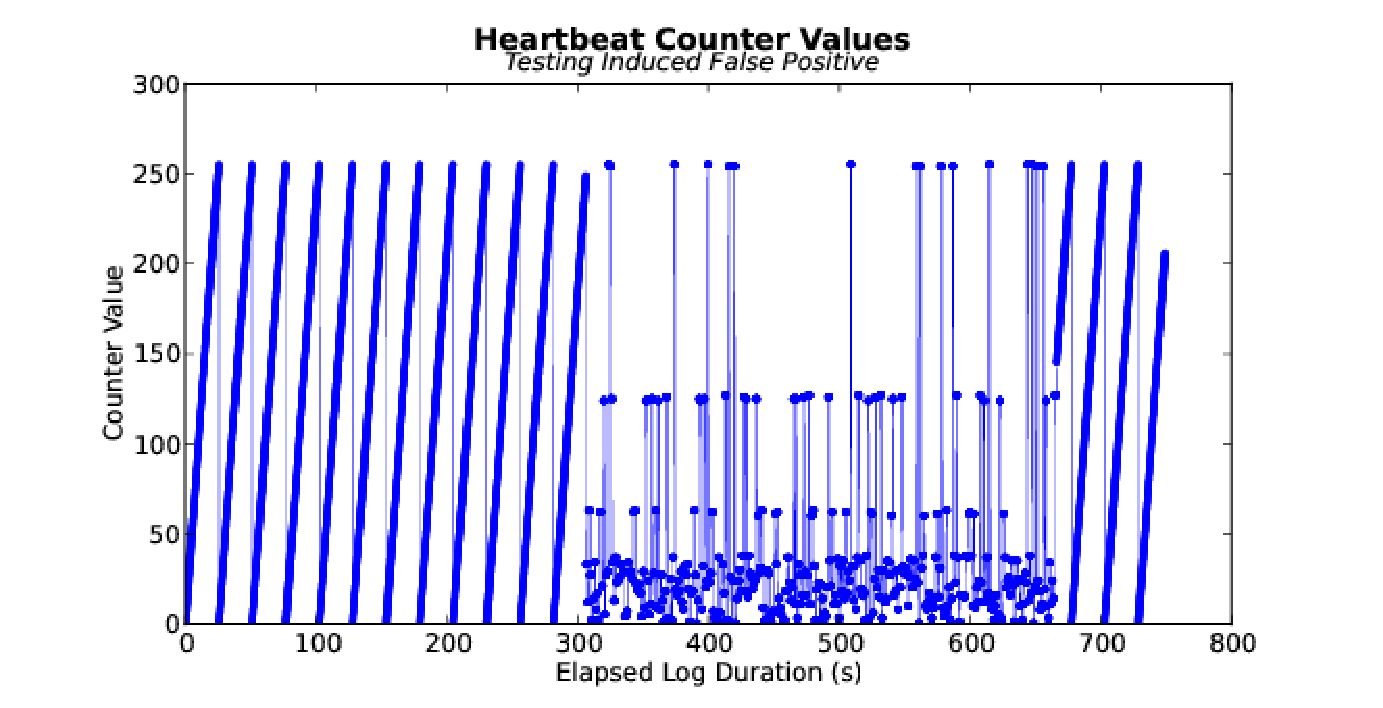
\includegraphics[width=4.5in]{img/hb2}
\caption{Bad heartbeat counter values \label{fig:eval:hb_badcounter}}
\end{figure}

%This was expected as these violations had been found with an offline monitoring tool previously.
The monitor also reported violations of the legal transition rules, but these, similar to the heartbeat counter violation, also turned out to be false positives triggered by message injections by the robustness testing harness. Since the monitor checks network state, if we perform testing that directly affects the values seen on the network (such as injection/interception of network messages) we may detect violations which are created by the testing framework rather than the system. 
%
%This is a common issue when using monitors as a test oracle with some sort of fault or behavior injection -- the monitor needs to know which state is from the test and which is from the system. 
Information about the test configurations can be used to filter out these types of false positives which arise from test-controlled state.
%These types of false positives can be filtered out by using the test configurations to keep track of what system properties are being affected by the testing. 
This type of filtering can be automated if the test information can be input to the monitor, either directly on the network (e.g., adding a message value to injected messages) or through a side-channel (i.e., building a testing-aware monitor).

%%@RV cutting
% detection time
%Comparing the violation messages from the monitor with the actual network state we can see the monitor's detection speed. 
%The deteection time for the monitor should approximately be the monitor's period plus the time to perform the monitoring and the time to send the detection message once the violation is detectable. 
%This is approximately two monitoring periods (given that the time to send a high priority message is negligable). This bears out in the replay testing, where the violation messages come approximately 555ms after the last good heartbeat message, which is a 55ms response time and close to double the monitor's 25ms period.



